% Chapter headings / Heading 1
\chapter{Chaptername}

% Heading 2
\section{Section Name}

% Heading 3
\section{Sub section 3}


% To make bullets
\begin{itemize}
\item Here is item 1
\item Here is item 2
\item here is item 3
\end{itemize}


% To make numbers
\begin{enumerate}
\item number item 2
\item number item 3
\item number item 4
\end{enumerate}

% Index of specific words used. If you find a specific word that you think people will be looking for add
\index{specific word}


“   ” ’


% Tables
% Use the table generator at http://www.tablesgenerator.com/latex_tables#

% To enable the tables to be only the width of text use tabularx instead of tablular. From the generated table, simply replace 

%\begin{table}[h]
%\centering
\begin{tabular}{lll}

\end{tabular}
%\caption{My caption}
%\label{my-label}
%\end{table}

with

%\begin{table}[h]
%\centering
\begin{tabularx}{\textwidth}{l X l} % Where the letters represent the                                           number of columns


\end{tabularx}
%\caption{My caption}
%\label{my-label}
%\end{table}

Note! l = left alight, c = center, r = right align and X = use available space


%To add a figure

\begin{figure}
\centering
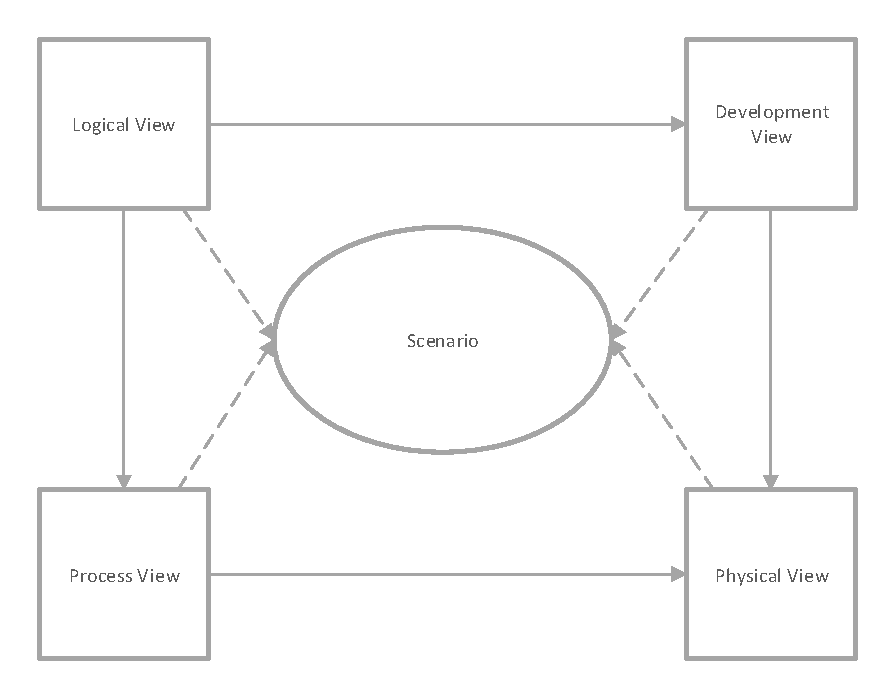
\includegraphics[width=\textwidth]{4plus1frameworksmall}
\caption{4 + 1 Framework}
\label{fig:4plus1frameworksmall}
\end{figure}